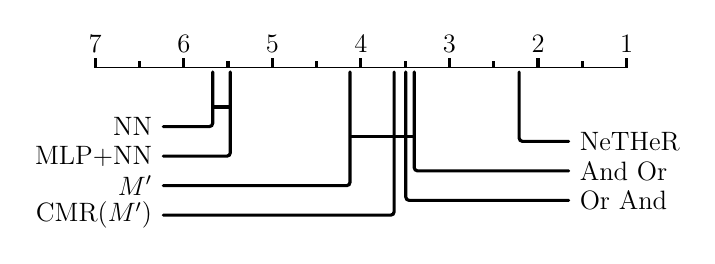
\begin{tikzpicture}[
  treatment line/.style={rounded corners=1.5pt, line cap=round, shorten >=1pt, line width=.5mm},
  treatment label/.style={font=\large},
  group line/.style={ultra thick},
  scale={0.8},
]

\begin{axis}[
  clip={false},
  axis x line={center},
  axis y line={none},
  axis line style={-},
  xmin={1},
  ymax={0},
  scale only axis={true},
  width={\axisdefaultwidth},
  ticklabel style={anchor=south, yshift=1.3*\pgfkeysvalueof{/pgfplots/major tick length}, font=\large},
  every tick/.style={draw=black, line width=.5mm},
  major tick style={yshift=.5*\pgfkeysvalueof{/pgfplots/major tick length}},
  minor tick style={yshift=.5*\pgfkeysvalueof{/pgfplots/minor tick length}},
  title style={yshift=\baselineskip},
  xmax={7},
  ymin={-4.5},
  height={5\baselineskip},
  xtick={1,2,3,4,5,6,7},
  minor x tick num={1},
  x dir={reverse},
]

\draw[treatment line] ([yshift=-2pt] axis cs:2.212962962962963, 0) |- (axis cs:1.6296296296296293, -2.5)
  node[treatment label, anchor=west] {NeTHeR};
\draw[treatment line] ([yshift=-2pt] axis cs:3.3981481481481484, 0) |- (axis cs:1.6296296296296293, -3.5)
  node[treatment label, anchor=west] {And Or};
\draw[treatment line] ([yshift=-2pt] axis cs:3.4930555555555554, 0) |- (axis cs:1.6296296296296293, -4.5)
  node[treatment label, anchor=west] {Or And};
\draw[treatment line] ([yshift=-2pt] axis cs:3.625, 0) |- (axis cs:6.256944444444444, -5.0)
  node[treatment label, anchor=east] {CMR($M'$)};
\draw[treatment line] ([yshift=-2pt] axis cs:4.122685185185185, 0) |- (axis cs:6.256944444444444, -4.0)
  node[treatment label, anchor=east] {$M'$};
\draw[treatment line] ([yshift=-2pt] axis cs:5.474537037037037, 0) |- (axis cs:6.256944444444444, -3.0)
  node[treatment label, anchor=east] {MLP+NN};
\draw[treatment line] ([yshift=-2pt] axis cs:5.673611111111111, 0) |- (axis cs:6.256944444444444, -2.0)
  node[treatment label, anchor=east] {NN};
\draw[group line] (axis cs:3.3981481481481484, -2.3333333333333335) -- (axis cs:4.122685185185185, -2.3333333333333335);
\draw[group line] (axis cs:5.474537037037037, -1.3333333333333333) -- (axis cs:5.673611111111111, -1.3333333333333333);

\end{axis}
\end{tikzpicture}